% -*- latex -*-
% FILE: "/home/evmik/jobs/wm/2011_spring_Analog_Electronics_252/final_exam/questions/output_impedance_of_fancy_opamp_amplifiers.tex"
% LAST MODIFICATION: "Thu, 05 May 2011 12:14:47 -0400 (evmik)"
% (C) 2011 by Eugeniy Mikhailov, <evgmik@gmail.com>
% $Id:$

\question{}
In this problem assume that you have an ideal Op-amp (the open loop gain $A=\infty$).
	\begin{parts}
		\part
		Consider the circuit below \\
		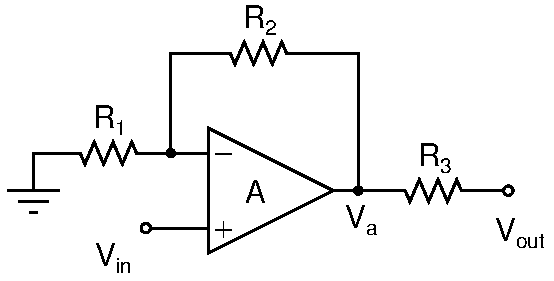
\includegraphics[height=1in]{./schematics/noninv_ampl_with_output_resistor}\\
		\begin{subparts}
			\subpart[5]
			Express $V_a$ and $V_{out}$ as function of $V_{in}$ and circuit
			components assuming no load connected.
			\vskip .8in
			\subpart[5]
			Assume that dummy load with resistance $R_L$ is
			connected to the output. Which of the voltages
			$V_a$ or $V_{out}$ depend on $R_L$?
			\vskip .8in
			\subpart[5]
			Using above find the output impedance of this
			circuit.
			\vskip .8in
		\end{subparts}

		\part
		Consider the circuit below \\
		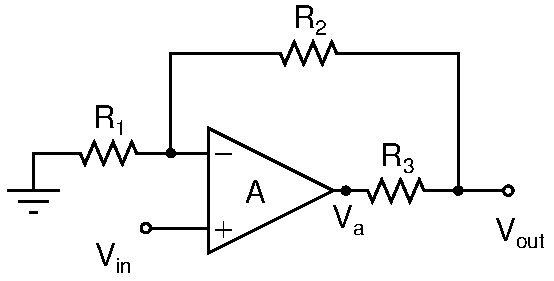
\includegraphics[height=1in]{./schematics/noninv_ampl_with_output_resistor_in_feedback}\\
		\begin{subparts}
			\subpart[5]
			Express $V_a$ and $V_{out}$ as function of $V_{in}$ and circuit
			components assuming no load connected.
			\vskip .8in
			\subpart[5]
			Assume that dummy load with resistance $R_L$ is
			connected to the output. Which of the voltages
			$V_a$ or $V_{out}$ depend on $R_L$? Hint: it is
			easier to find $V_{out}$ if you consider the
			current through $R_2$ and $R_1$.
			\vskip .8in
			\subpart[5]
			Using above find the output impedance of this
			circuit.
			\vskip .8in
		\end{subparts}
	\end{parts}

	\pagebreak
